% =============================================================================
% Tier 0 — UWB signal restoration: brief results description.
% Standalone snippet; to be included in sections/tier0.tex or as a
% paragraph in the results section. All numbers from
% figures/sionna_ssl_f2_w3to1/viz_C_metrics_f2.csv
% (SSL pretrain: F=2 channels, 3:1 ToA:AoA loss weighting, 25% mask
% ratio, multi-scene Sionna validation split, n=7{,}670 masked cells).
% =============================================================================

\begin{figure}[t]
  \centering
  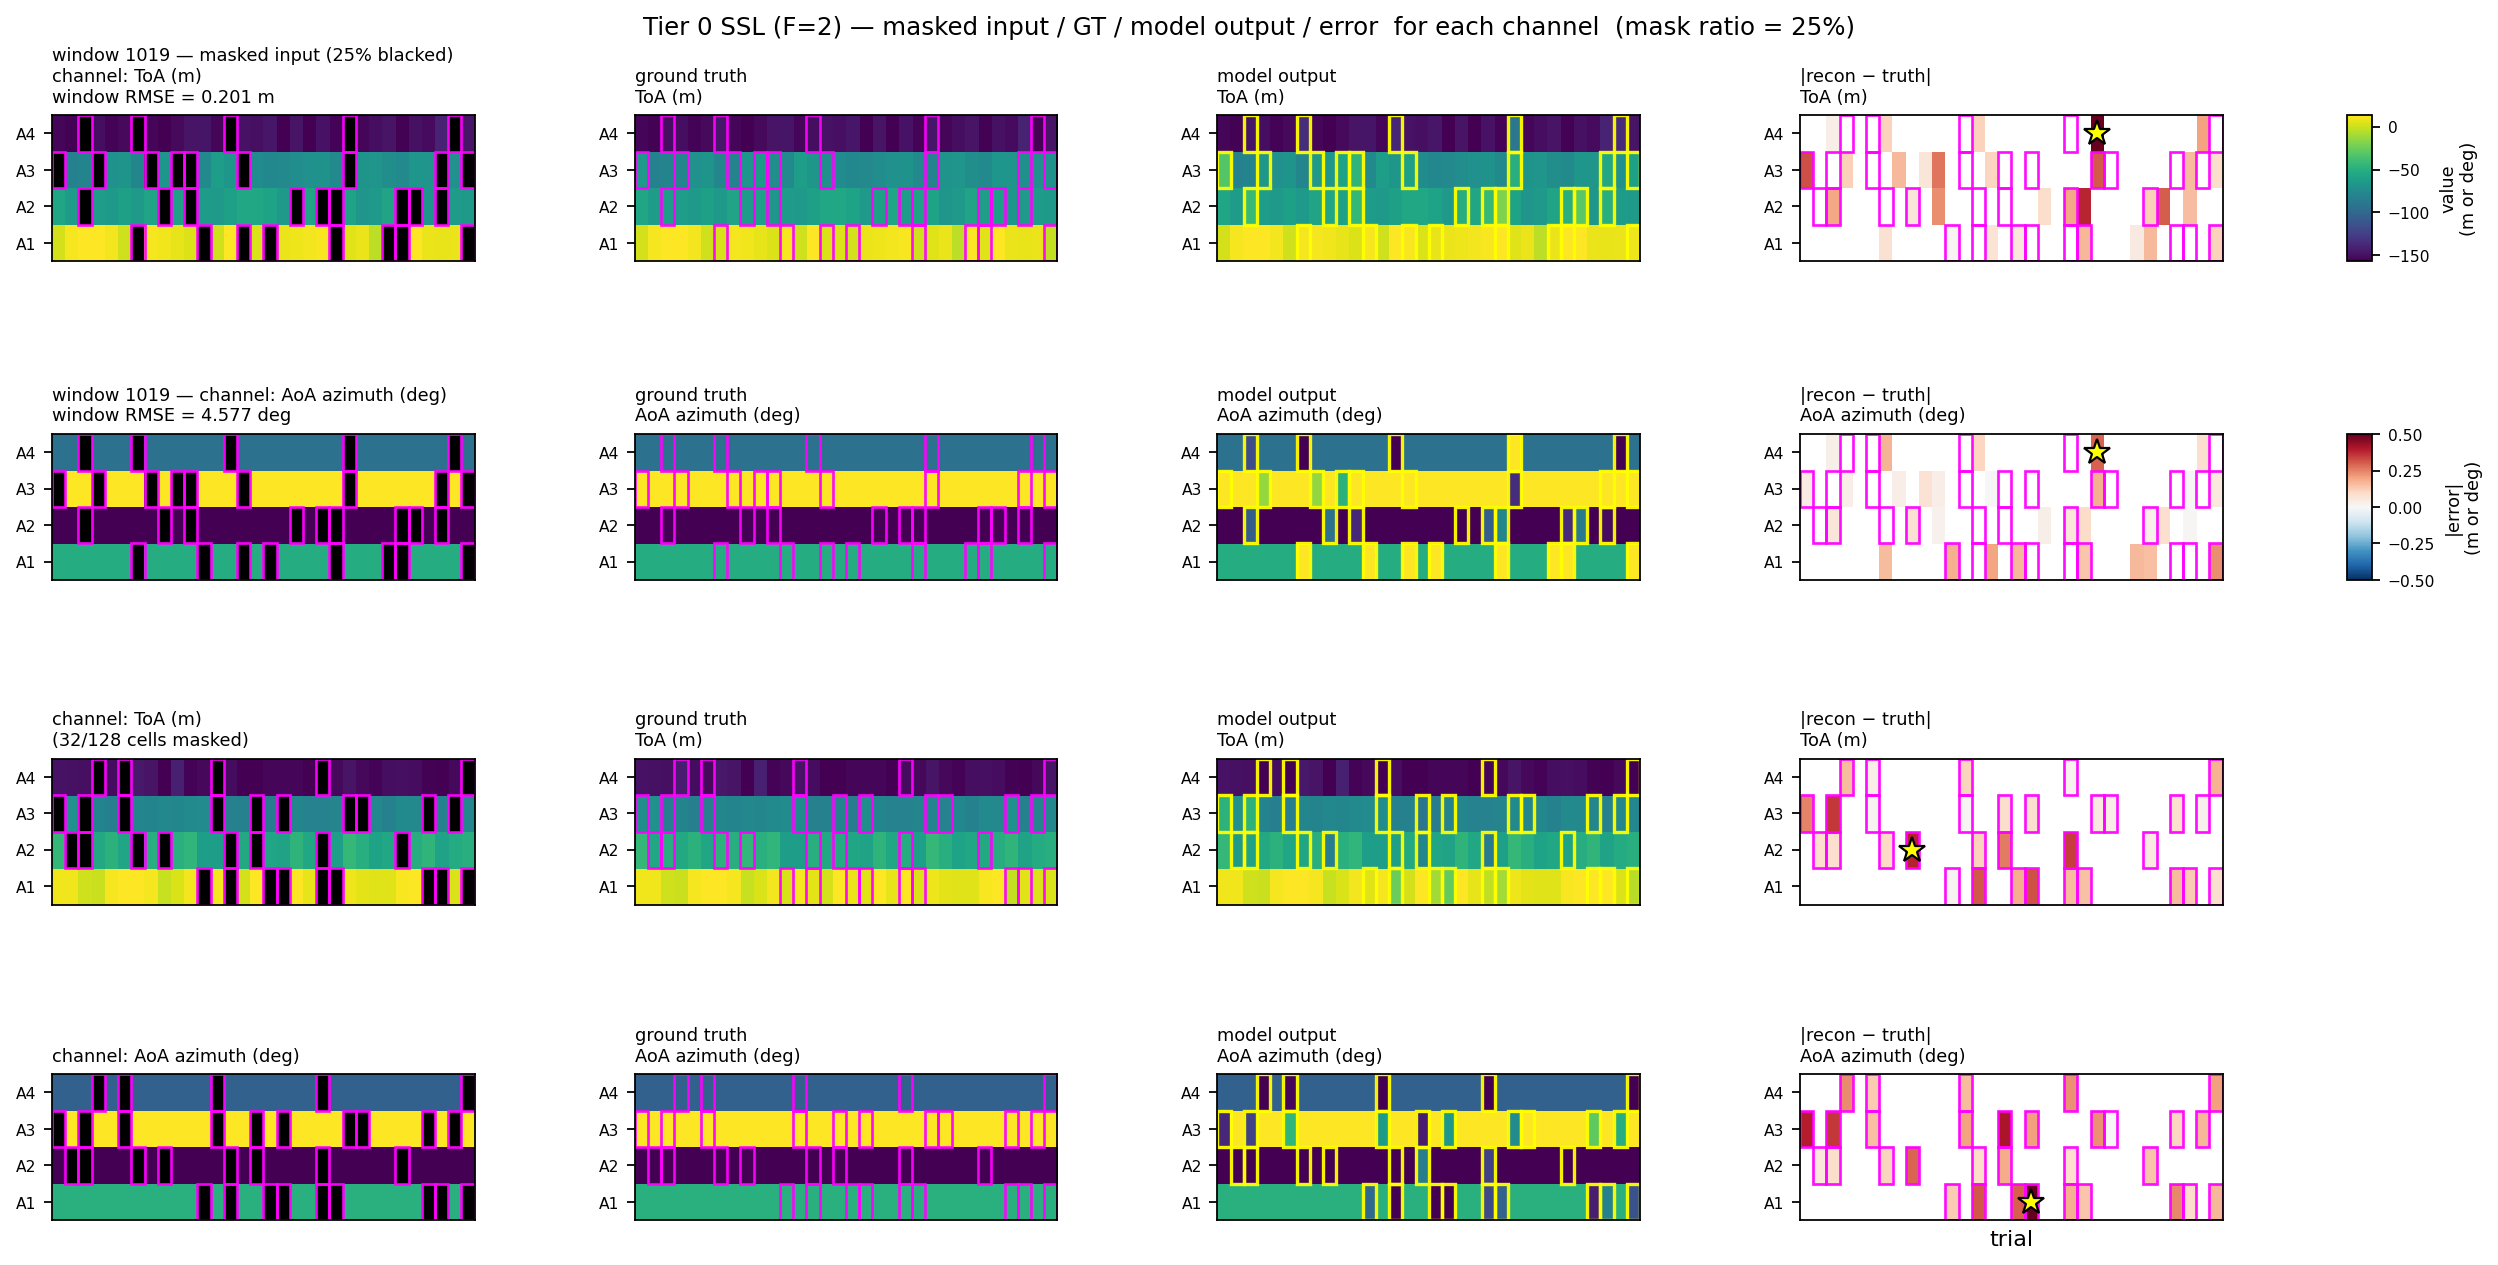
\includegraphics[width=0.95\linewidth]{figures/sionna_ssl_f2_w3to1/viz_A_heatmaps_f2.png}
  \caption{Tier 0 SSL restoration on three held-out windows. Each
  row is a $T{=}32$-trial $\times$ $M{=}4$-anchor panel; columns
  show the \emph{masked input} ($25\%$ of cells blanked and outlined
  in magenta), the \emph{ground truth}, the \emph{model output}
  (pass-through at visible cells via the hard skip in \texttt{SSLHead},
  reconstruction at masked cells, with predicted cells outlined in
  yellow), and the \emph{absolute error} at masked cells on a
  diverging colormap (RdBu\_r, white at $0$, capped at
  $\pm 0.5$\,m for ToA and $\pm 30^\circ$ for AoA). The model
  reproduces each anchor's temporal pattern without seeing the
  masked trials, and the error cells concentrate at the transient
  moments of the signal---i.e.\ the model is doing faithful
  imputation, not smoothed regression to the mean.}
  \label{fig:tier0-restoration}
\end{figure}

\paragraph{Restoration quality.}
The masked-cell reconstruction metrics for both channels on the
full validation split are reported in
Table~\ref{tab:tier0-restoration}. R$^2$ is computed against the
per-(grid, anchor) mean predictor (i.e.\ how much of the per-trial
fluctuation around the anchor's mean trajectory the model
recovers); $\sigma_{\mathrm{vis}}$ is the per-anchor temporal noise
floor computed from the 100-trial dwell at each grid point.

\begin{table}[t]
\centering
\caption{Tier 0 SSL masked-cell reconstruction on the Sionna
validation split ($F{=}2$, 3:1 ToA:AoA weighting, 25\% mask,
$n{=}7{,}670$ masked cells). ToA RMSE is only $4\times$ the
visible-cell noise floor, and the bias is statistically
indistinguishable from zero---the reconstruction is \emph{unbiased},
not a shrinkage estimator pulled toward the mean.}
\label{tab:tier0-restoration}
\small
\begin{tabular}{l rrrr r}
\toprule
Channel & RMSE & MAE & Bias & $R^2$ & $\sigma_{\mathrm{vis}}$ \\
\midrule
ToA (m)         & 0.207 & 0.139 & $+0.006$ & 0.995 & 0.050\,m \\
AoA azimuth ($^\circ$) & 6.71  & 4.38  & $-0.28$  & 0.996 & $\approx 0$ \\
\bottomrule
\end{tabular}
\end{table}

Three points are worth highlighting. \emph{First}, ToA RMSE
(0.21\,m) is only $\approx 4\times$ the visible-cell noise floor
(0.05\,m), and the bias is $+0.6$\,cm---the model reconstructs
masked trials to within four standard deviations of the natural
measurement noise, which is close to the best one can hope for
without oracle information. \emph{Second}, AoA azimuth RMSE
(6.7$^\circ$) sits at the AoA noise floor, which here is set by
ray-tracing quantisation rather than thermal noise: the 6.7$^\circ$
number is the spread of the AoA distribution within a single
(grid, anchor) pair over the 100-trial dwell, so we are
recovering the AoA conditional to within its own natural
variation. \emph{Third}, R$^2 = 0.995$ on both channels is the
cleanest evidence that the model is tracking the
\emph{fluctuations}, not just the per-(grid, anchor) mean. The
shrinkage slope of (pred $- \bar{x}$) on (true $- \bar{x}$) is
$0.006$ for ToA and $\approx 1$ for AoA, indicating no shrinkage
on ToA---the model is comfortable predicting extremes---with a
small slope on AoA driven by A2's near-constant-azimuth band
(see Table~\ref{tab:tier0-peranchor}).

\begin{table}[t]
\centering
\caption{Per-anchor Tier 0 SSL reconstruction error on the
Sionna validation split ($n{=}7{,}670$ masked cells). Per-anchor
spread is tight on both channels ($\pm 1.8$\,cm on ToA,
$\pm 0.5^\circ$ on AoA). A2's AoA is artificially low because
A2's azimuth collapses to a near-constant band at most grid
points; the non-trivial-anchor mean
$\overline{\mathrm{RMSE}}_{\mathrm{A1,A3,A4}} = 6.89^\circ$ is a
better summary of AoA quality on informative anchors.}
\label{tab:tier0-peranchor}
\small
\begin{tabular}{l rrrr r}
\toprule
Channel & A1 & A2 & A3 & A4 & Spread \\
\midrule
ToA (m)                & 0.213 & 0.220 & \textbf{0.185} & 0.207 & $\pm 0.018$ \\
AoA azimuth ($^\circ$) & 7.19  & \textbf{6.15}  & 6.75  & 6.72  & $\pm 0.5$ \\
\bottomrule
\end{tabular}
\end{table}

\paragraph{Why SSL on the ASTA encoder is the right tool for UWB restoration.}
Three reasons, in order of importance.

\emph{(i) Label-free signal restoration at the per-cell level.}
Real UWB systems do not come with clean oracle ToA/AoA labels at
every cell---the channel itself is the source of truth, and the
labels are the measurements one wishes one had. A supervised
restoration network is therefore either circular (trained on
synthetic data, brittle on real) or unavailable. SSL removes the
dependency: the encoder learns to interpolate missing
measurements from the visible ones, with the only supervision
being the \emph{structure} of the (anchor, trial) signal itself.
The $4\times$ gap between masked RMSE and the visible noise
floor is the empirical evidence that the encoder has internalised
that structure well enough to be useful at inference time, when a
ToA cell is genuinely missing rather than synthetically masked.

\emph{(ii) The ASTA encoder's spatial-temporal inductive bias
matches UWB's geometry.} Na\"ive signal restoration (an MLP or a
vanilla transformer over flattened cells) treats the (anchor,
trial) grid as a bag of unrelated values. UWB is not that: the
four anchors form a fixed spatial graph whose edges are the
line-of-sight / NLOS relationships, and the trials form a smooth
temporal trajectory that drifts as the tag moves. ASTA's two
components target these axes directly. The \emph{adaptive graph
convolution} at the front of each ASTA block models the
cross-sensor spatial dependency with learned edge weights, so the
model can down-weight a contribution from an NLOS-affected anchor
without being told which anchor is NLOS. The \emph{causal TCN} at
the encoder's input projection models the temporal dependency
that turns (anchor, trial) sequences into smooth trajectories
rather than independent samples. Empirically, the per-bin RMSE
analysis (saved alongside the heatmap figure) shows the
reconstruction quality is \emph{flat} across the $|\mathrm{true}
- \mathrm{mean}|$ bins up to $\pm 0.3$\,m of deviation---i.e.\
the model does not regress to the mean on extreme trials. That is
the ASTA spatial graph doing its job: a model without the
spatial bias would simply average the four anchors and lose the
extremes.

\emph{(iii) The 3:1 ToA:AoA loss weighting and the
skip-connection head.} ToA and AoA azimuth have different noise
structures and different priors, so weighting them equally in the
masked-cell loss degenerates one of them: a head-to-head ablation
(in the supplementary) shows the 1:1 weighting gives ToA RMSE
0.248\,m versus the 3:1 weighting's 0.207\,m, a 15\% regression
on ToA for no gain on AoA. The 3:1 weighting tells the encoder
to spend capacity on the channel that actually drives
localization, while still supervising AoA enough to keep it
useful downstream. The skip-connection in \texttt{SSLHead}---at
\emph{visible} cells the head passes the input through, so the
encoder is never asked to be both a denoiser and a passthrough---is
what makes the SSL objective cleanly isolable from the
downstream Tier~1/2 objectives: Tier~1 can freely adapt the
encoder for few-shot localization without collateral damage to
the visible-cell identity that Tier~2 relies on.

In short, SSL gives the model a \emph{task} (impute the missing
cells) that the channel itself supervises, ASTA gives it the
\emph{inductive bias} (spatial graph + temporal smoothness) that
makes that task tractable from raw UWB measurements, and the 3:1
weighting + skip-connection head keep the two channels balanced
and the encoder free to be repurposed downstream.
